% ==================================================
% CHAPTER 3: Using cosmic muon data for alignment studies
% ==================================================

\chapter{Using cosmic muon data for alignment studies}

The cosmic muon data collected is high in statistics, and the clean trail of ionization left by the muons leaves a clean signal.

% --------------------------------------------------
\section{Measuring alignment using cosmics data}
% --------------------------------------------------

Misalignments can be modeled as passive transformations. Ideally, a misalignment model would be chosen and the parameters, like a global offset and rotation for each layer, calculated. To understand the potential of cosmic muon data, it is useful to define a local offset. For each area of a strip layer, the local offset is defined to be the offset of the strip pattern in that area with respect to the nominal geometry.  Local offsets systematically change the strip that is hit by a muon passing through the area. The \package{tgc\_analysis/CosmicsAnalysis} software assumes the nominal geometry, so the recorded muon y-position ($y_{cluster}$) is shifted opposite to the local offset ($d_{local}$},
% Maybe useful sentence?: The local offset is a result of the non-conformities in the strip pattern etching and inter-layer misalignments.
\begin{equation}
    y_{cluster} = y_{nom} - d_{local}
    \label{eqn:local_translation}
\end{equation}
% Maybe useful sentence?: The true position of individual cosmic muons is not known, and in the analysis the four detector planes float with respect to a software-implemented origin that is not associated with a fixed physical location.
ignoring other factors that could affect the cluster position (like resolution). The local offset is unknown, and there was no external reference to measure where the muon would have passed through if the geometry was nominal, $y_{nom}$. The result is that only relative alignment parameters can be extracted. The minimal relative coordinate system assumes that two sTGC layers are fixed~\cite{lefebvre_thesis}. The hits on the two fixed layers are used to create a track that can be interpolated or extrapolated to the other two layers. The residual of track $i$, $\Delta_i$ is defined as,
\begin{equation}
    \Delta_i = y_{i,hit} - y_{i,track}
    \label{eqn:residual}
\end{equation}

Track residuals are affected by the local offset in the area of each layer's hit, as shown in figure~\ref{fake_event_display}. 

\begin{figure}
    \centering
    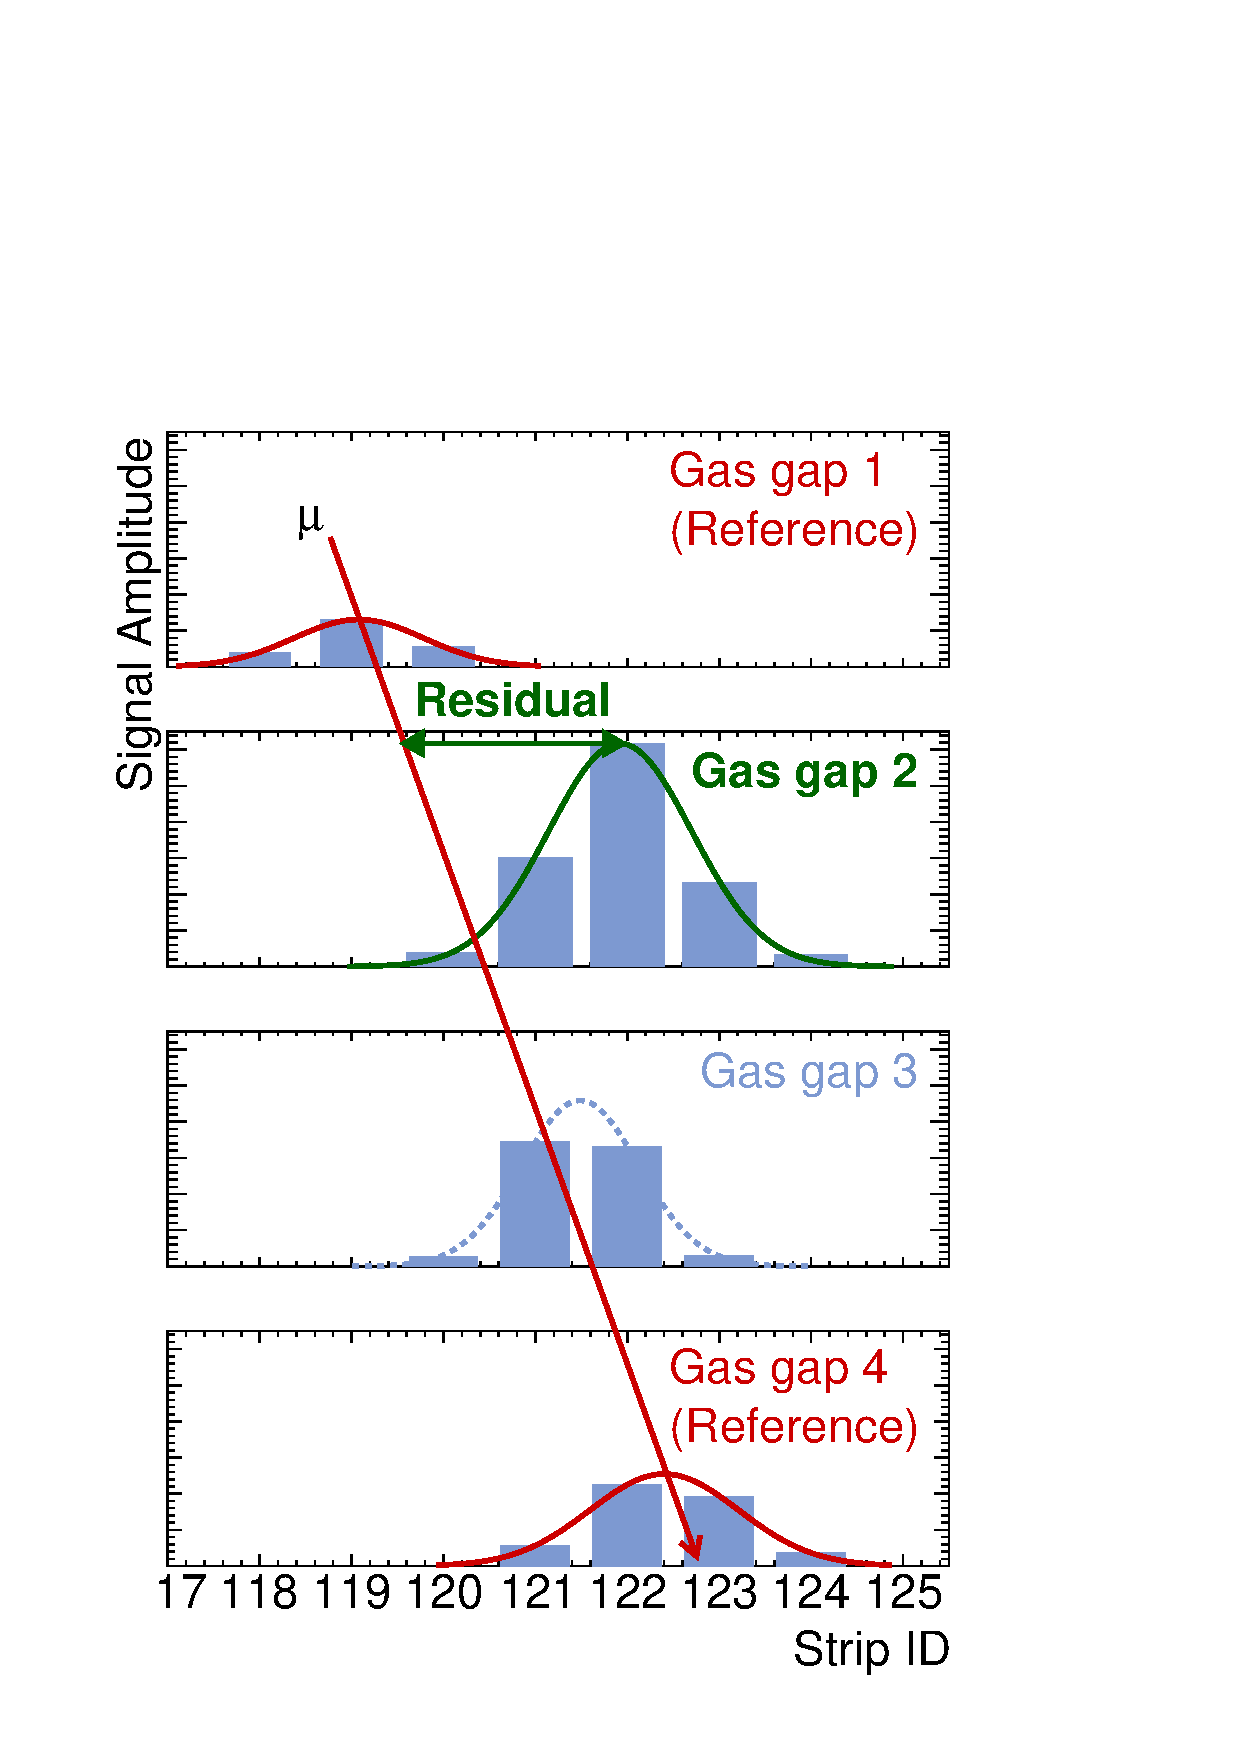
\includegraphics[width = \textwidth]{figures/figure_fake_event_display.pdf}
    \caption{Representation of a muon event recorded by an sTGC. The clusters are fit with a Gaussian and the mean is taken as the hit position. A track is built from the chosen reference layers, 1 and 4, and the residual calculated on layer 2.}
    \label{fig:fake_event_display}
\end{figure}

A single The mean of residuals for all tracks in a local area will be shifted systematically by the local misalignments between layers~\cite{lefebvre_thesis}. 

